\documentclass[aspectratio=169]{beamer}

%%%%%
%%%%%
%%%%%     DEFINE THE THEME USED
%%%%%
%%%%%

\usetheme{jc}

%%%%%
%%%%%
%%%%%     LIST OF PACKAGES USED
%%%%%
%%%%%

\graphicspath{{imgs/}}

\usepackage[utf8]{inputenc}
\usepackage[T1]{fontenc}

\usepackage[]{amsmath, amssymb, amsfonts}
\usepackage[]{bm}

\usepackage[]{graphicx}

\usepackage{tikz}
\usetikzlibrary{shapes}

%%%%%
%%%%%
%%%%%     INFO ABOUT THE PRESENTATION
%%%%%
%%%%%

\title{On the importance of low-dimensional structures for data-driven modeling}
\author[JC]{Jean-Christophe Loiseau}
\date[]{May, 13\textsuperscript{th} 2022}

%%%%%
%%%%%
%%%%%     PRESENTATION
%%%%%
%%%%%

\begin{document}

\begin{frame}
  \titlepage
\end{frame}

%% \begin{frame}[t, c]{blabla}
%%   \vfill

%%   \centering
  
%%   This is a test

%%   \vfill
  
%%   \begin{tcolorbox}[enhanced, coltitle=black, coltext=white, colback=black, title=My title, frame style tile={width=\paperwidth}{background.jpg}]
%%     Hello
%% \end{tcolorbox}
  
%%   \vfill
%% \end{frame}

\begin{frame}{Who am I ?}
  \vfill
  \begin{minipage}{.68\textwidth}
    \begin{itemize}
    \item Maître de Conférences in Fluid Dynamics and Applied Math.

      \bigskip

    \item Machine-learning enthusiast with application to engineering systems.

      \bigskip

    \item Data-efficient models with guarantees of optimality or interpretability.
    \end{itemize}
  \end{minipage}%
  \hfill
  \begin{minipage}{.28\textwidth}
    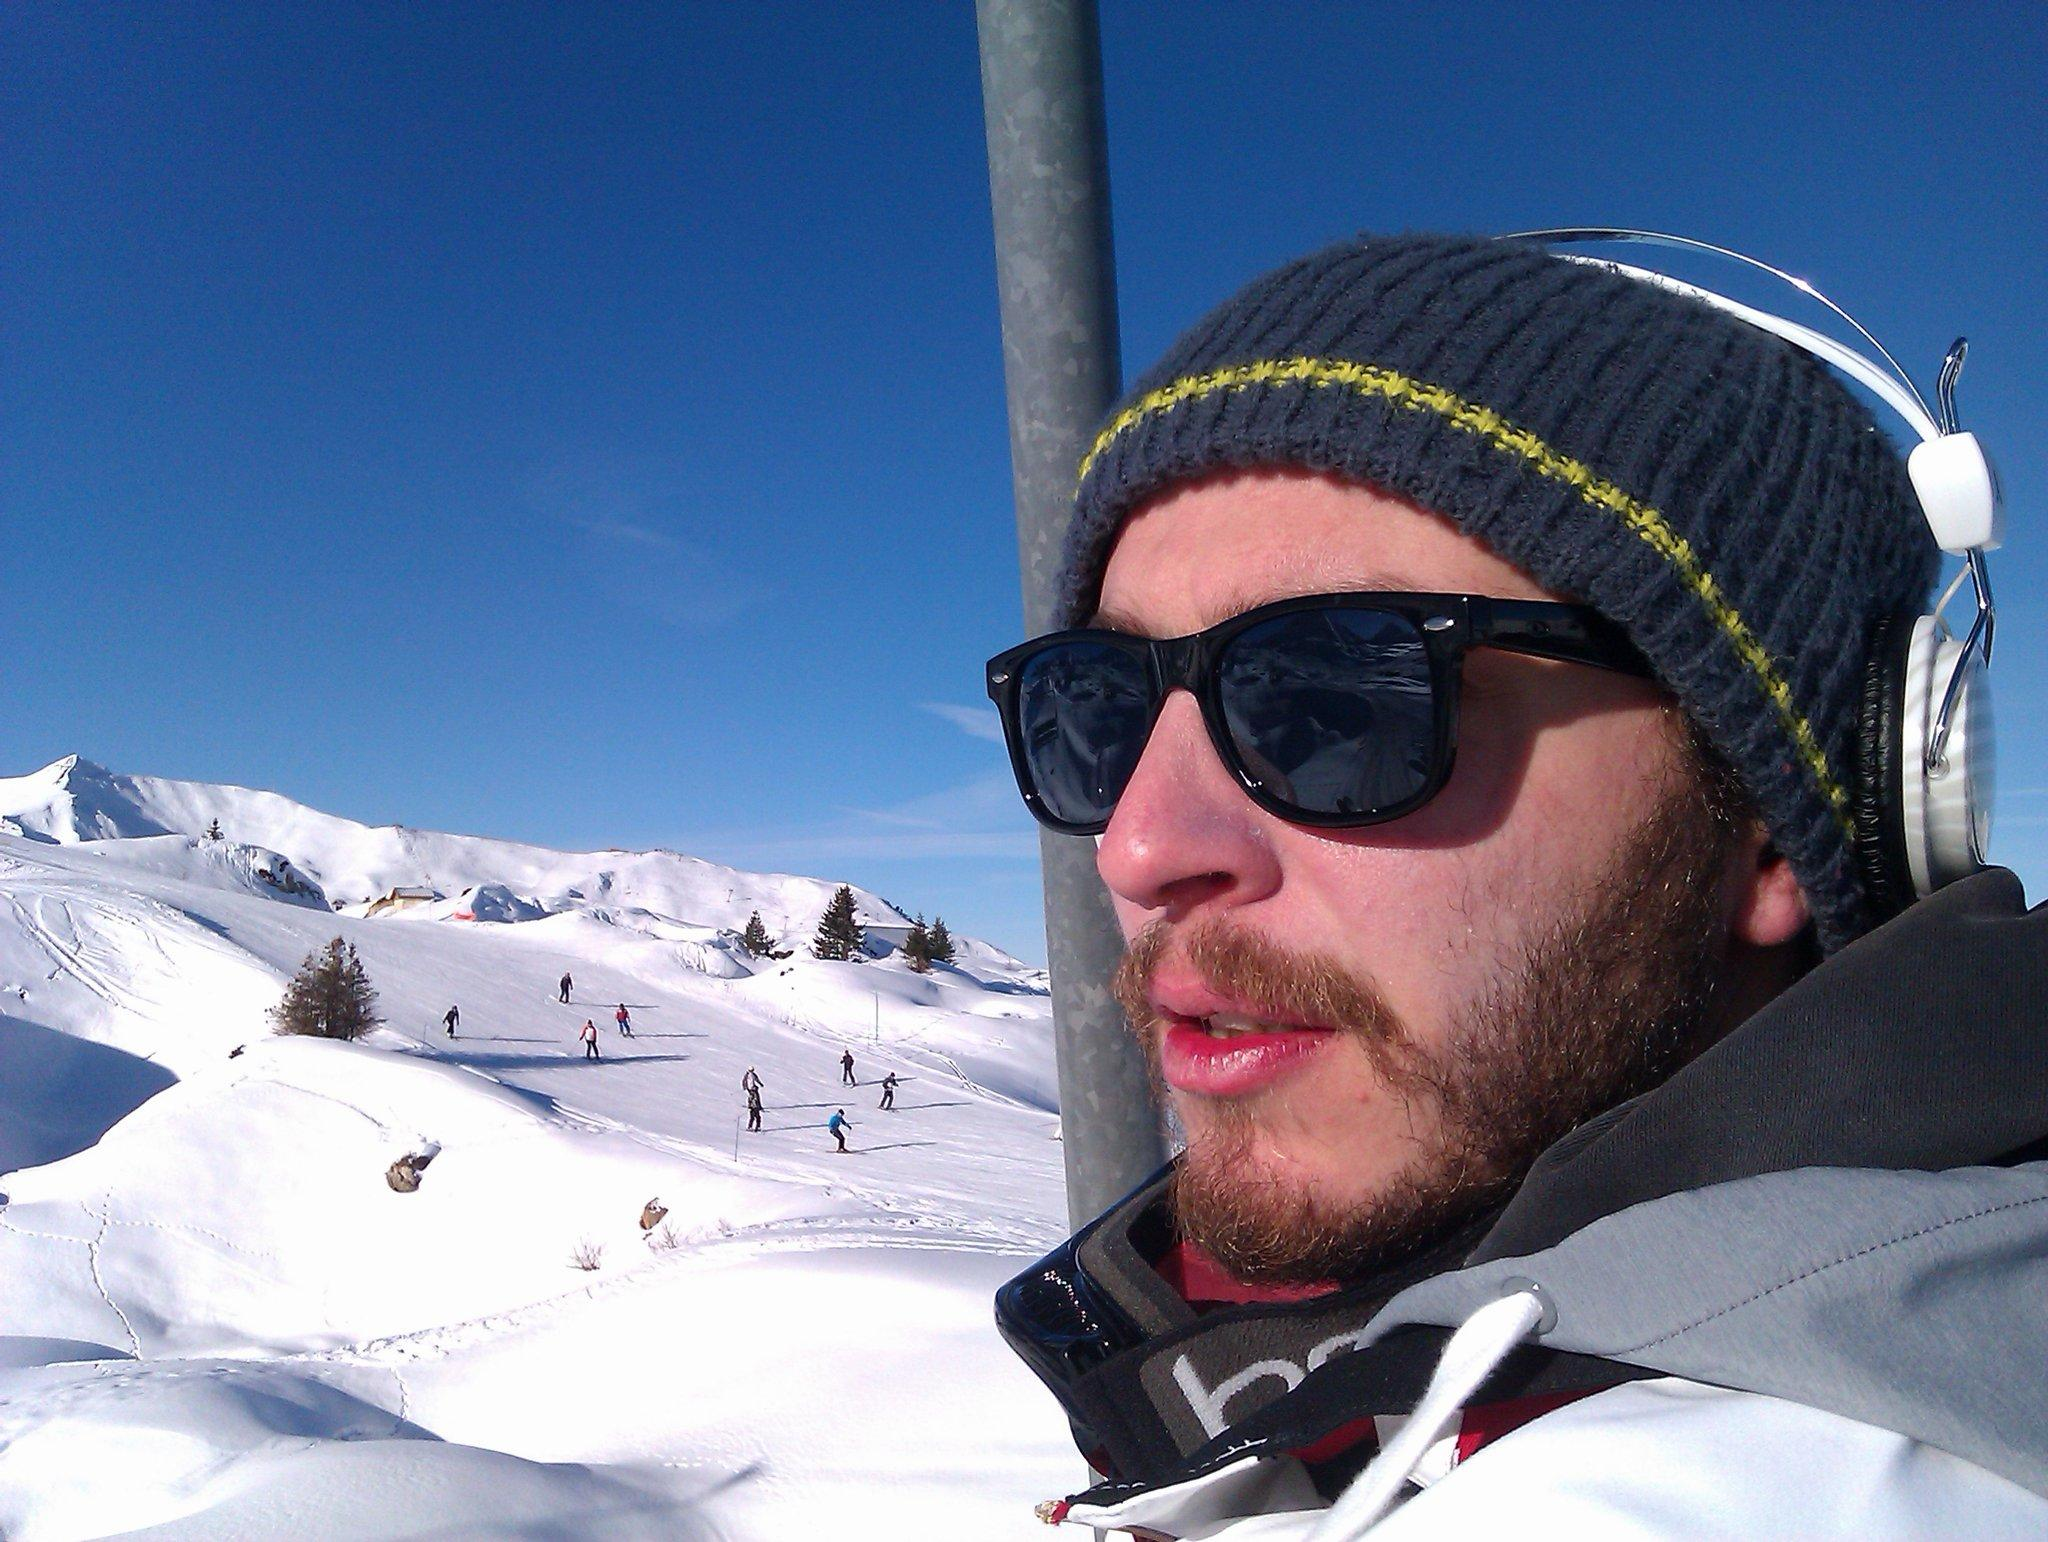
\includegraphics[width=\textwidth]{myself}
  \end{minipage}
  
  \vfill
\end{frame}

{
  \setbeamercolor*{background canvas}{bg=white}

\begin{frame}%{A gallery of fluid motion}
  \vfill
  \begin{minipage}{.68\textwidth}
    \centering
    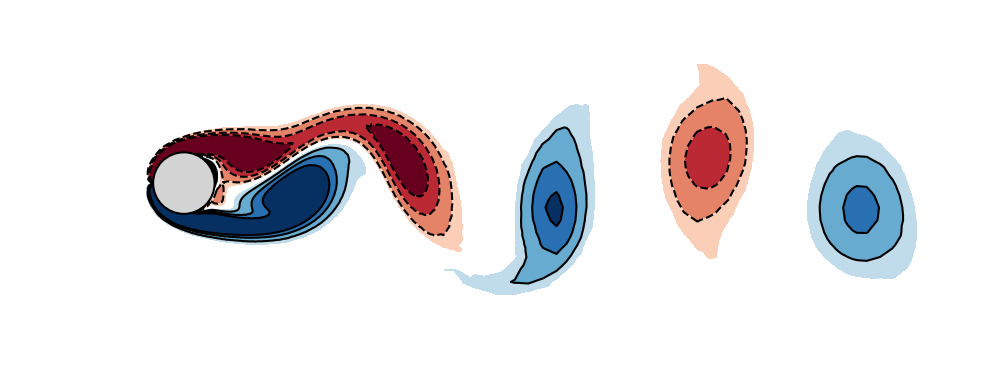
\includegraphics[width=\textwidth]{snapshot_re125_0}
    
    {\small \textcolor{black}{Aerodynamics}}

    \bigskip
    
    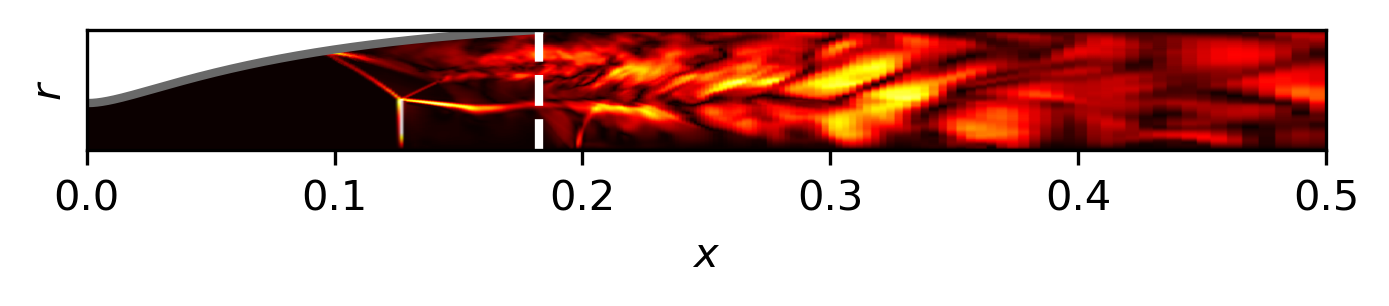
\includegraphics[width=\textwidth]{tic_m=1_fourier_mode_snapshot}

    {\small \textcolor{black}{Rocket science}}
  \end{minipage}%
  \hfill
  \begin{minipage}{.28\textwidth}
    \centering
    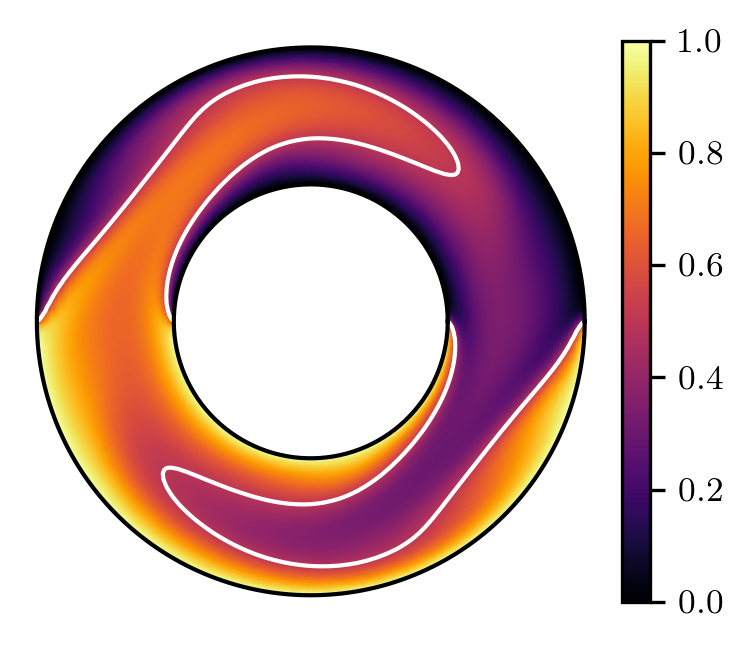
\includegraphics[width=\textwidth]{temperature_field_00000}

    {\small \textcolor{black}{Heat exchange}}
  \end{minipage}
  
  \vfill
\end{frame}
}

\begin{frame}{N.\ Wiener's classification}
  \centering
  \vfill

  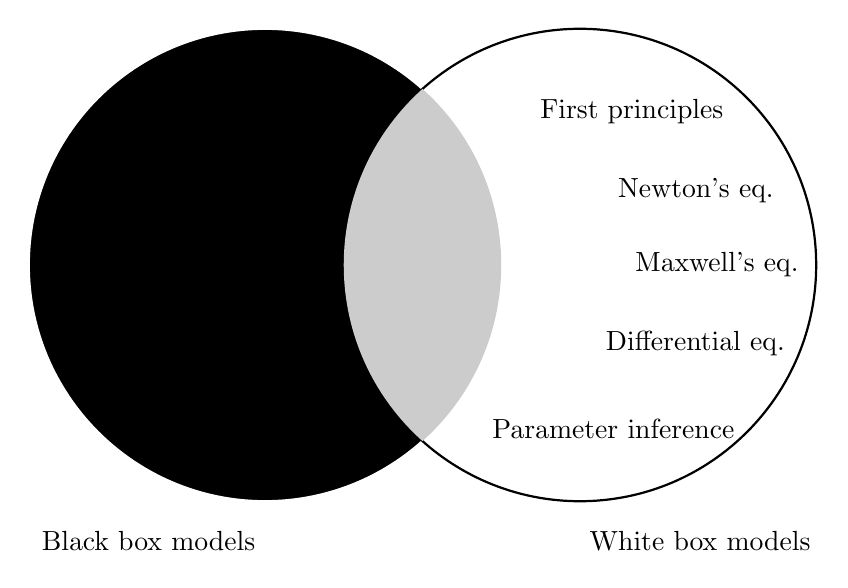
\begin{tikzpicture}
    %\draw[help lines, step=1] (-7, -3) grid (7, 3);

    \draw[thick, white, fill=black] (-2, 0) circle (3);
    \draw[thick, black,fill=white] (2, 0) circle (3);

    \begin{scope}
      \clip (-2, 0) circle (3);
      \clip (2, 0) circle (3);
      \fill[thick, black, fill=gray!40] (0, 0) circle (3);
    \end{scope}

    \node[anchor=east] at (-2, -3.5) {Black box models};
    \node[anchor=west] at (2, -3.5) {White box models};

    \node at (-2, 0) (A) {};
    \path (A) ++(135:2.75) node[anchor=west] {Feedforward nets};
    \path (A) ++(160:2.95) node[anchor=west] {Reinforcement};
    \path (A) ++(170:2.8) node[anchor=west] {learning};
    \path (A) ++(195:2.95) node[anchor=west] {Image classification};
    \path (A) ++(220:2.95) node[anchor=west] {Model-free inference};


    \node at (2, 0) (B) {};
    \path (B) ++(45:2.75) node[anchor=east] {\textcolor{black}{First principles}};
    \path (B) ++(20:2.75) node[anchor=east] {\textcolor{black}{Newton's eq.}};
    \path (B) ++(0:2.9) node[anchor=east] {\textcolor{black}{Maxwell's eq.}};
    \path (B) ++(-20:2.9) node[anchor=east] {\textcolor{black}{Differential eq.}};
    \path (B) ++(-45:2.95) node[anchor=east] {\textcolor{black}{Parameter inference}};

  \end{tikzpicture}
  
  \vfill
\end{frame}

\begin{frame}{Example: Face recognition}
  two faces with arrows
\end{frame}

\begin{frame}{Example: Face recognition}
  overview figure of the SIAM paper
\end{frame}

\begin{frame}{Example: System identification}
  
\end{frame}

\section{A brief overview of SVD}
\begin{frame}
  \sectionpage
\end{frame}

\begin{frame}
  \vfill

  
  \begin{tcolorbox}[
    enhanced,
    coltitle=black,
    coltext=white,
    colback=black,
    title=Singular value decomposition,
    frame style tile={width=\paperwidth}{background.jpg}
    ]
    
    \large
    \[
      \begin{aligned}
        \bm{Av}_i & = \sigma_i \bm{u}_i \\
        \bm{A}^T \bm{u}_i & = \sigma_i \bm{v}_i
      \end{aligned}
    \]
    
  \end{tcolorbox}

  \bigskip
  
  Generalization of the \emph{eigenvalue decomposition} to \textbf{non-square matrices} by E. Beltrami (1873) and C. Jordan (1874).
  The first efficient numerical algorithm was developed by G.\ Golub \emph{et al.} in the late 1960s.
  
  \vfill
\end{frame}

\end{document}
